% example from https://tex.stackexchange.com/questions/388800/horizontal-and-vertical-braces-below-and-next-to-a-tabular-table


\documentclass[presentation, aspectratio=1610, 12pt, t]{beamer}
\usepackage{tikz}
\usetikzlibrary{arrows,
                calc,
                decorations.pathreplacing,
                calligraphy,% had to be after decorations.pathreplacing
                matrix,
                positioning
                }

\begin{document}
\begin{frame}[fragile]
\[
    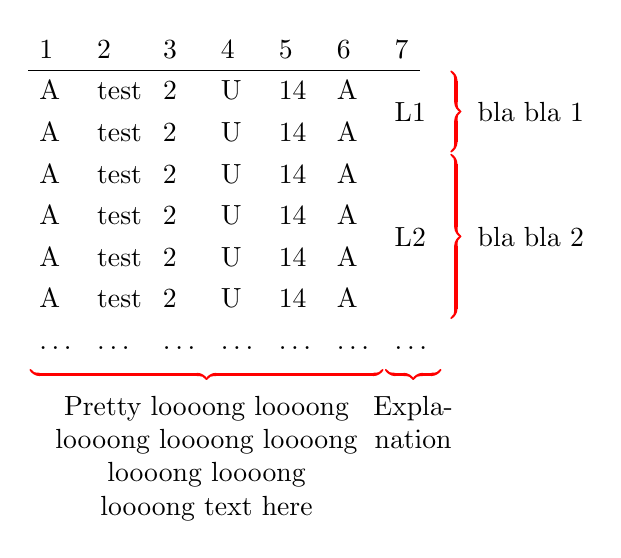
\begin{tikzpicture}[
node distance = 0pt,
    BC/.style = {
        decorate,
        decoration={calligraphic brace, amplitude=1.2mm,
        pre =moveto, pre  length=0.75pt,
        post=moveto, post length=0.75pt,
        raise=1mm,
        #1},% for mirroring of brace
        very thick,
        pen colour={red}% black ...
                  },
  BC/.default = mirror,
    LN/.style = {inner xsep=4pt, outer sep=0pt},
                        ]
\matrix (m) [matrix of nodes, inner sep=0pt,
             nodes={text depth=0.8ex, text height=1em, %minimum width=5ex,
                    inner ysep=1pt, inner xsep=4pt, outer sep=0pt, anchor=west},
             nodes in empty cells,
             column sep=-\pgflinewidth,
             row sep= -\pgflinewidth,
             ]
{
    1   & 2     & 3     & 4     & 5     & 6     & 7     \\
    A   & test  & 2     & U     & 14    & A     &       \\
    A   & test  & 2     & U     & 14    & A     &       \\
    A   & test  & 2     & U     & 14    & A     &       \\
    A   & test  & 2     & U     & 14    & A     &       \\
    A   & test  & 2     & U     & 14    & A     &       \\
    A   & test  & 2     & U     & 14    & A     &       \\
\dots   & \dots & \dots & \dots & \dots & \dots & \dots \\
};
\node[LN,right=of m-2-6.south -| m-1-7.west] {L1};
\node[LN,right=of m-5-6.south -| m-1-7.west] {L2};
\draw           (m-1-1.south west) -- (m-1-7.south east);
\draw[BC={}]    (m-2-7.north -| m.east) --
                    node[right=3mm] {bla bla 1}
                (m-3-7.south -| m.east);
\draw[BC={}]    (m-4-7.north -| m.east) --
                    node[right=3mm] {bla bla 2}
                (m-7-7.south -| m.east);
%
\draw[BC]   let \p1 = ($(m-1-1.west)-(m-1-6.east)$),
                \n1 = {veclen(\x1,\y1)} in
            (m-8-1.south west) --
                node[text width=\n1, align=center,
                     below=3mm] {Pretty loooong loooong loooong loooong loooong loooong loooong loooong text here}
            (m-8-6.south east)
                    ;
\draw[BC]   (m-8-7.south west) --
                node[align=center, below=3mm] {Expla- \\
                                               nation}
            (m-8-7.south east);
    \end{tikzpicture}
\]
\end{frame}
\end{document}